\documentclass{beamer}

\usefonttheme{professionalfonts} % using non standard fonts for beamer
\usefonttheme{serif} % default family is serif

%\usepackage{hyperref}

%\usepackage{minted}

\usepackage{animate}

\usepackage{graphicx}

\def\Put(#1,#2)#3{\leavevmode\makebox(0,0){\put(#1,#2){#3}}}

\usepackage{color}

\usepackage{tikz}

\usepackage{amssymb}

\usepackage{enumerate}


\newcommand\blfootnote[1]{%

  \begingroup

  \renewcommand\thefootnote{}\footnote{#1}%

  \addtocounter{footnote}{-1}%

  \endgroup

}

\makeatletter

%%%%%%%%%%%%%%%%%%%%%%%%%%%%%% Textclass specific LaTeX commands.

 % this default might be overridden by plain title style

 \newcommand\makebeamertitle{\frame{\maketitle}}%

 % (ERT) argument for the TOC

 \AtBeginDocument{%

   \let\origtableofcontents=\tableofcontents

   \def\tableofcontents{\@ifnextchar[{\origtableofcontents}{\gobbletableofcontents}}

   \def\gobbletableofcontents#1{\origtableofcontents}

 }

%%%%%%%%%%%%%%%%%%%%%%%%%%%%%% User specified LaTeX commands.

\usetheme{Malmoe}

% or ...

\useoutertheme{infolines}

\addtobeamertemplate{headline}{}{\vskip2pt}



\setbeamercovered{transparent}

% or whatever (possibly just delete it)

\makeatother

\begin{document}
\title[SDCEL report]{A Scalable DCEL implementation}
\author[AC]{Andres Calderon}
\institute[UCR]{University of California, Riverside}
\makebeamertitle
\newif\iflattersubsect

% \AtBeginSection[] {
%   \begin{frame}<beamer>
%     \frametitle{Outline} 
%     \tableofcontents[currentsection]  
%   \end{frame}
%   \lattersubsectfalse
% }

\AtBeginSubsection[] {
  \begin{frame}<beamer>
    \frametitle{Outline} 
    \tableofcontents[currentsubsection]  
  \end{frame}
}


\begin{frame}{Evaluation Plan...}
    \centering 
    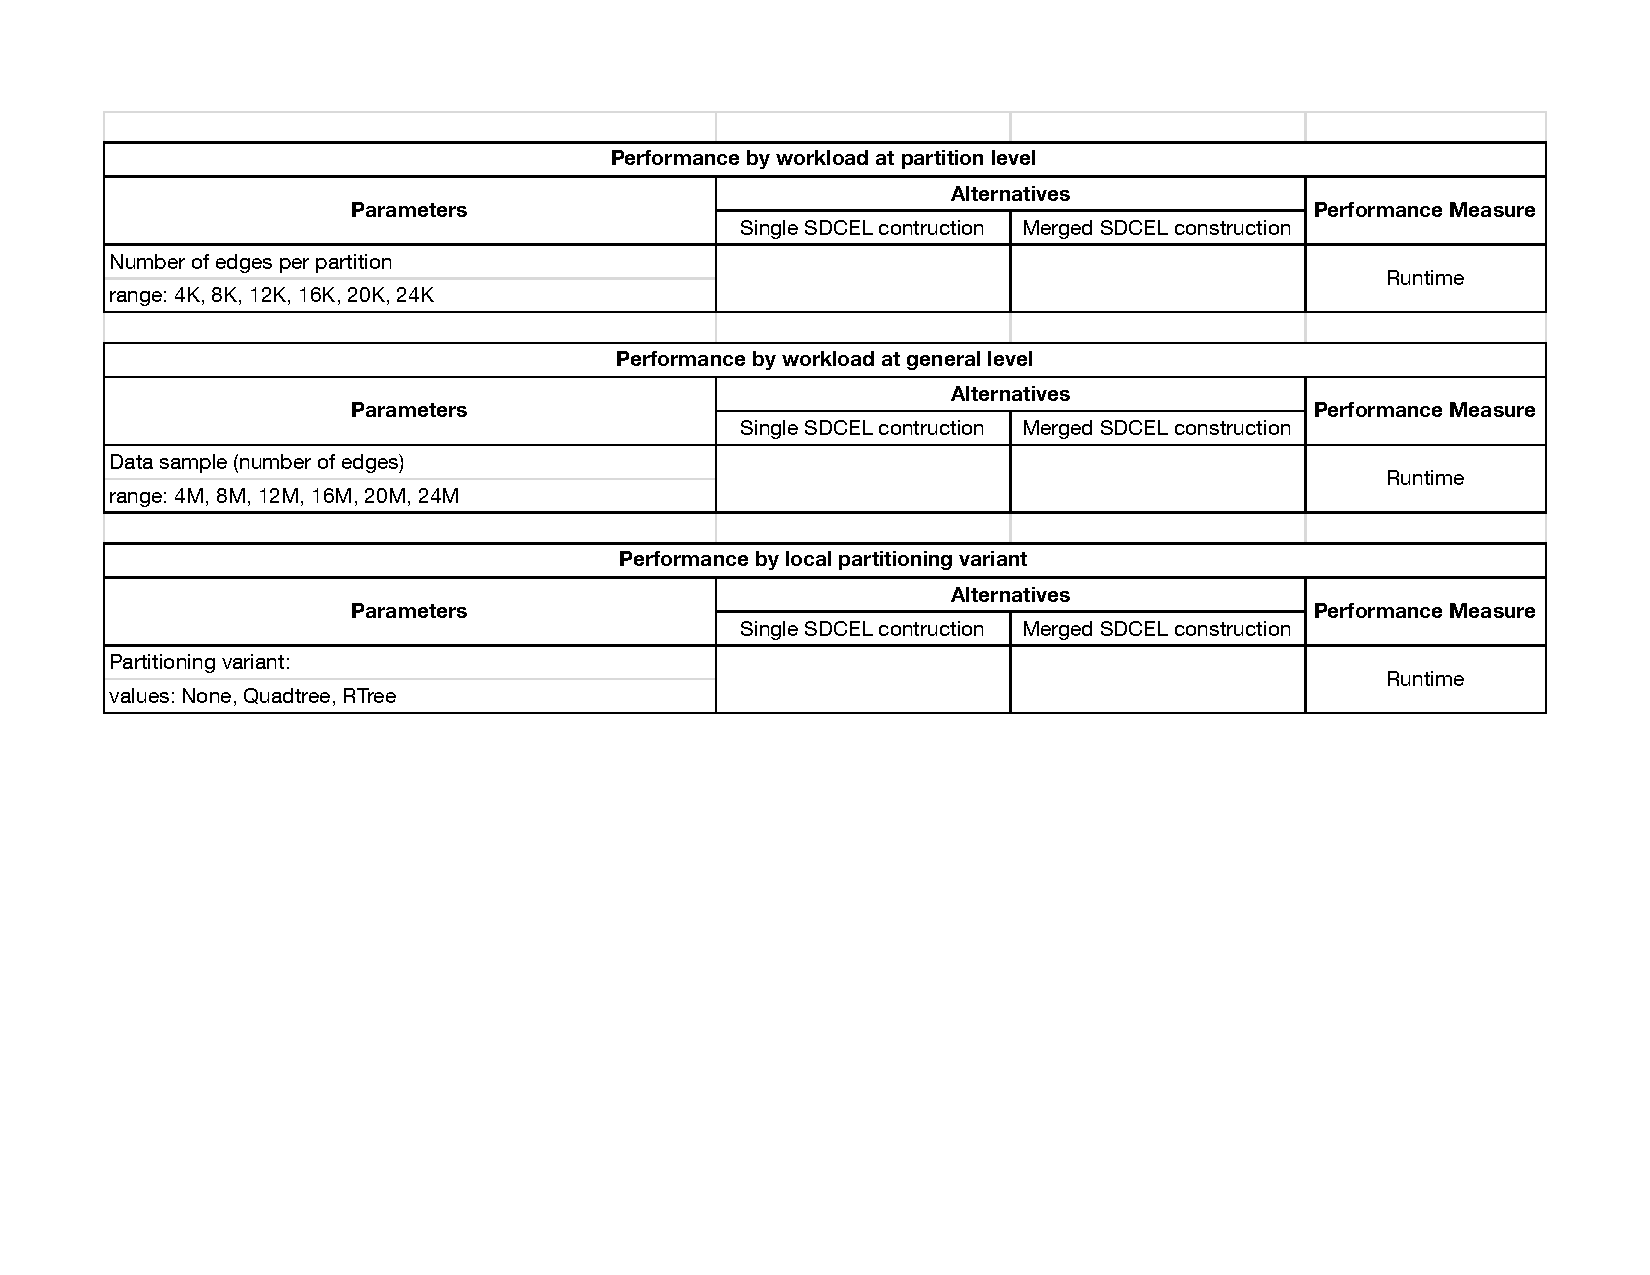
\includegraphics[trim=0cm 2cm 0cm 0cm, clip, width=1\textwidth]{figures/ep}
\end{frame}

\begin{frame}{Fixing balancing issues...}
    \centering 
    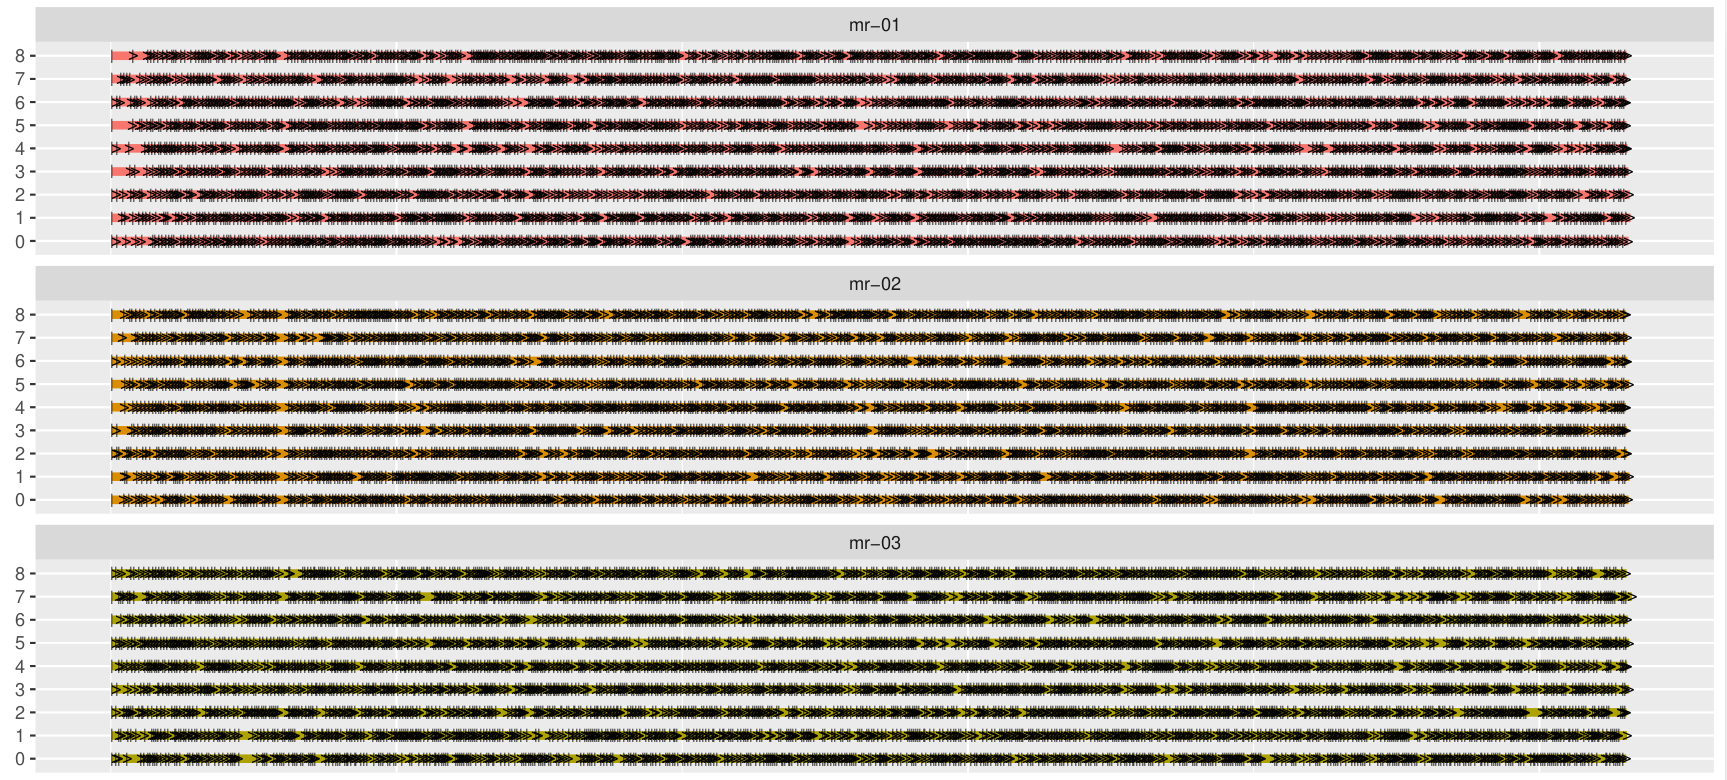
\includegraphics[width=1\textwidth]{figures/balance}
\end{frame}

\begin{frame}{Collecting partition stats...}
    \centering 
    \begin{table}[ht]
    \centering
    \begin{tabular}{rlrrr}
    \hline
    & avg\_edges & max\_edges & max\_entries & partitions \\ 
    \hline
    1 & 2K & 7390       & 650   & 33754 \\ 
    2 & 3K & 10146     & 950   & 23182 \\ 
    3 & 4K & 13136     & 1250 & 17662 \\ 
    4 & 5K & 16390     & 1550 & 14131 \\ 
    5 & 6K & 19184     & 1850 & 11836 \\ 
    6 & 7K & 23014     & 2150 & 10099 \\ 
    7 & 8K & 25836     & 2500 & 8713 \\ 
    8 & 9K & 28771     & 2800 & 7873 \\ 
    9 & 10K & 32534   & 3150 & 7006 \\ 
    10 & 11K & 36072 & 3450 & 6391 \\ 
    11 & 12K & 38526 & 3800 & 5830 \\ 
    12 & 13K & 41746 & 4100 & 5359 \\ 
    13 & 14K & 44856 & 4350 & 5038 \\ 
    14 & 15K & 47880 & 4650 & 4681 \\ 
    \hline
    \end{tabular}
    \end{table}    
\end{frame}

\begin{frame}{Running experiments...}
    \centering 
    \begin{table}[ht]
    \centering
    \begin{tabular}{rlrrr}
    \hline
    & avg\_edges & max\_edges & mean\_duration & max\_duration \\ 
    \hline
    1 & 2K & 7390 & 0.10 & 5.00 \\ 
    2 & 3K & 10146 & 0.20 & 6.60 \\ 
    3 & 4K & 13136 & 0.38 & 10.40 \\ 
    4 & 5K & 16390 & 0.48 & 12.40 \\ 
    5 & 6K & 19184 & 0.62 & 16.00 \\ 
    6 & 7K & 23014 & 0.80 & 24.20 \\ 
    7 & 8K & 25836 & 0.98 & 25.60 \\ 
    8 & 9K & 28771 & 1.00 & 38.00 \\ 
    9 & 10K & 32534 & 1.00 & 40.80 \\ 
    10 & 11K & 36072 & 2.00 & 51.00 \\ 
    11 & 12K & 38526 & 2.00 & 55.80 \\ 
    12 & 13K & 41746 & 2.00 & 75.20 \\ 
    13 & 14K & 44856 & 2.00 & 69.60 \\ 
    14 & 15K & 47880 & 2.60 & 83.80 \\ 
    \hline
    \end{tabular}
    \end{table}   
\end{frame}

\begin{frame}{Running experiments...}
    \centering 
    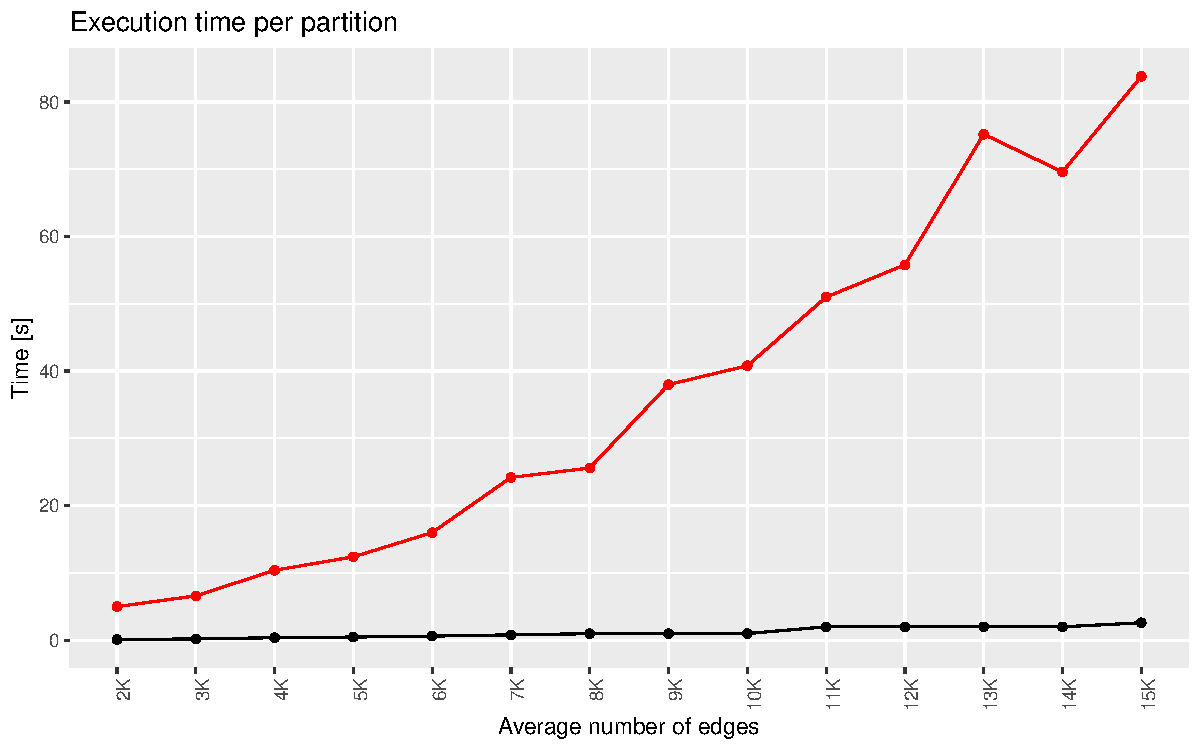
\includegraphics[width=1\textwidth]{figures/Run}
\end{frame}

\end{document}
